\chapter{I parxshenxgaLa utatxragaLu - {\rm I}}

\begin{enumerate}
  \renewcommand{\labelenumi}{\rm(\theenumi)}
    \itemsep=2pt
\item $1^2+ 2^2 = 1+4=5$

\item $5+4=9$

\item $1^2+2^2+3^2 = 1+4+9 =14$

\item $1^2 + 2^2 + 3^2+4^2 = 1+4+9+16 = 30$

\item $8$

\item $6$

\item $12$

\item $5$ kaNaRgaLu

\item $10$

\item
  ~

  \vskip -0.4cm
  
  \begin{tabular}[t]{l}
 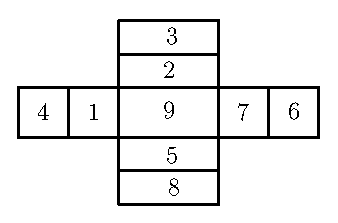
\includegraphics{src/figures/ans10.eps}
\end{tabular}

  \newpage

\item 
~

  \vskip -0.6cm
  \begin{tabular}[t]{c}
\centering
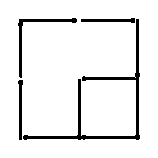
\includegraphics{src/figures/ans11.eps}
\end{tabular}
\smallskip

\item 
~

  \vskip -0.4cm
  
\begin{tabular}[t]{c}
\centering

\includegraphics{src/figures/ans12.eps}
\end{tabular}

\smallskip

\item 
~

  \vskip -0.5cm
  
\begin{tabular}[t]{c}
\centering
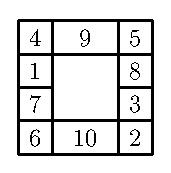
\includegraphics{src/figures/ans13.eps}
\end{tabular}

\item 
~

  \vskip -0.4cm
  
\begin{tabular}[t]{c}
\centering
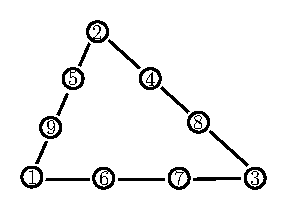
\includegraphics{src/figures/ans14.eps}
\end{tabular}

\item $360^{\circ}$

\item $5$

  \smallskip
  
\item 
~

  \vskip -0.5cm
  
\begin{tabular}[t]{c}
\centering
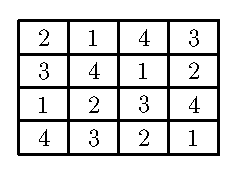
\includegraphics{src/figures/ans17.eps}
\end{tabular}

\newpage

\item 
~

  \vskip -0.5cm
  
\begin{tabular}[t]{c}
\centering
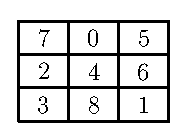
\includegraphics{src/figures/ans18.eps}
\end{tabular}

\medskip

\item 
~

  \vskip -0.5cm
  
\begin{tabular}[t]{c}
\centering
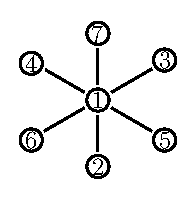
\includegraphics{src/figures/ans19.eps}
\end{tabular}

\medskip

\item 
~

  \vskip -0.5cm
  
\begin{tabular}[t]{c}
\centering

\includegraphics{src/figures/ans20.eps}
\end{tabular}

\medskip

\item 
~

  \vskip -0.5cm
  
\begin{tabular}[t]{c}
\centering
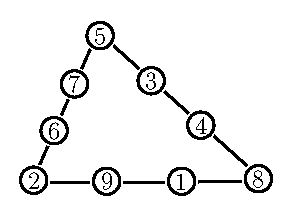
\includegraphics{src/figures/ans21.eps}
\end{tabular}

\medskip

\item $9+3+1=13$

  \medskip
  
\item 
~

  \vskip -0.5cm
  
\begin{tabular}[t]{c}
\centering
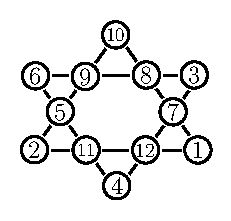
\includegraphics{src/figures/ans23.eps}
\end{tabular}

\item 
~

  \vskip -0.5cm
  
\begin{tabular}[t]{c}
\centering
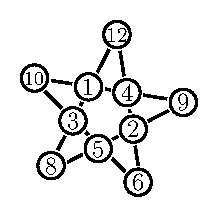
\includegraphics{src/figures/ans24.eps}
\end{tabular}

\bigskip
  \bigskip

\item 
~

  \vskip -0.6cm
  
\begin{tabular}[t]{c}
\centering
\includegraphics{src/figures/ans25.eps}
\end{tabular}

\bigskip
\bigskip

\item 
~

  \vskip -0.6cm
  
\begin{tabular}[t]{c}
\centering
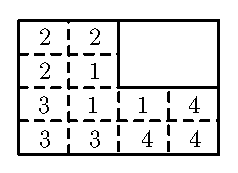
\includegraphics{src/figures/ans26.eps}
\end{tabular}

\bigskip
\bigskip

\item 
~
  \vskip -0.6cm
  
\begin{tabular}[t]{c}
\centering
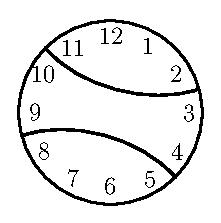
\includegraphics{src/figures/ans27.eps}
\end{tabular}

\vfill\eject

\item 
~

  \vskip -0.4cm
  
\begin{tabular}[t]{c}
\centering
\includegraphics{src/figures/ans28.eps}
\end{tabular}

\item $20$

\item 
~

  \vskip -0.4cm
  
\begin{tabular}[t]{c}
\centering
\includegraphics{src/figures/ans30.eps}
\end{tabular}

\item 
~

  \vskip -0.4cm
  
\begin{tabular}[t]{c}
\centering
\includegraphics{src/figures/ans31.eps}
\end{tabular}

\item 
~

  \vskip -0.4cm
  
\begin{tabular}[t]{c}
\centering
\includegraphics{src/figures/ans32.eps}
\end{tabular}

\item 
~

  \vskip -0.4cm
  
\begin{tabular}[t]{c}
\centering
\includegraphics{src/figures/ans33.eps}
\end{tabular}

\item 
~

  \vskip -0.5cm
  
\begin{tabular}[t]{c}
\centering
\includegraphics{src/figures/ans34.eps}
\end{tabular}
$ADB - BF - FE-ED-DF-FC-CEA$

\bigskip

\item 
~

  \vskip -0.5cm
  
\begin{tabular}[t]{c}
\centering
\includegraphics{src/figures/ans35.eps}
\end{tabular}

\bigskip

\item 
~

  \vskip -0.5cm
  
\begin{tabular}[t]{c}
\centering
\includegraphics{src/figures/ans36.eps}
\end{tabular}

\bigskip

\item 
~

  \vskip -0.5cm
  
\begin{tabular}[t]{c}
\centering
\includegraphics{src/figures/ans37.eps}
\end{tabular}

\bigskip
\bigskip

\item 
~

  \vskip -0.4cm
  
\begin{tabular}[t]{c}
\centering

\includegraphics{src/figures/ans38.eps}
\end{tabular}

\item 
~

  \vskip -0.4cm
  
\begin{tabular}[t]{c}
\centering
\includegraphics{src/figures/ans39.eps}
\end{tabular}

\bigskip

\item 
~

  \vskip -0.4cm
  
\begin{tabular}[t]{c}
\centering
\includegraphics{src/figures/ans40.eps}
\end{tabular}

\bigskip

\item 
~

  \vskip -0.4cm
  
\begin{tabular}[t]{c}
\centering
\includegraphics{src/figures/ans41.eps}
\end{tabular}

\bigskip

\item 
~

  \vskip -0.4cm
  
\begin{tabular}[t]{c}
\centering
\includegraphics{src/figures/ans42.eps}
\end{tabular}

\bigskip

\item 
~

  \vskip -0.4cm
  
\begin{tabular}[t]{c}
\centering
\includegraphics{src/figures/ans43.eps}
\end{tabular}

\item eraDU oMdeV
  
\item  $5$

\item eraDU oMdeV 

\item eraDaneyadu $300\%$ jAsitx tirxjayxda $4$ seM.miV
 
\end{enumerate}
